\chapter{Metodología}

A continuación hablaré de la gestión del proyecto y la metodología del desarrollo, así como del control de versiones y repositorio de este \ac{TFG}.

\section{Metodología del desarrollo}

Para el desarrollo del desarrollo de este proyecto he usado la metodología \textit{Kanban}, una metodología ágil basada en tableros y etiquetas. Para ello usaremos \textit{Trello}, una herramienta de gestión de proyectos que utiliza esta metodología de manera cómoda y práctica.

\subsection{¿Qué es Kanban?}

\textit{\textbf{Kanban}} es una metodología ágil creada hace muchos años en el seno de \textit{Toyota} y que ha sido usada durante décadas para mantener la línea de producción.
\\

Se basa en las siguientes ideas:

\begin{itemize}
	\item Permite tener una visualización del trabajo realizado.
	\begin{itemize}
		\item Divide todo el trabajo en ítems o tarjetas.
		\item Utiliza diferentes columna para poder visualizar en que parte del flujo de trabajo está cada ítem.
	\end{itemize}
	\item Mide y gestiona el flujo de trabajo.
	\item Permite identificar oportunidades de mejora.
\end{itemize}


Es una metodología muy útil y adecuada para este proyecto, ya que está pensada para equipos pequeños y que permite cambios imprevistos con mayor facilidad que otras metodologías.
\\

Un ejemplo de uso de esta metodología es el siguiente:

\begin{enumerate}
	\item Se crean tarjetas con tareas a realizar.
	\item Se mueven esas tarjetas a la columna \textit{Working} una vez que se empieza a trabajar con ellas.
	\item Cuando se termina con esa tarea se mueve la tarjeta a la columna \textit{Done}.
	\item Por último, se vuelve a escoger tareas en las que trabajar y se repite los pasos anteriores, así hasta la finalización del proyecto.
\end{enumerate}
	
\section{Gestión del proyecto}

\begin{figure}
	\begin{center}
		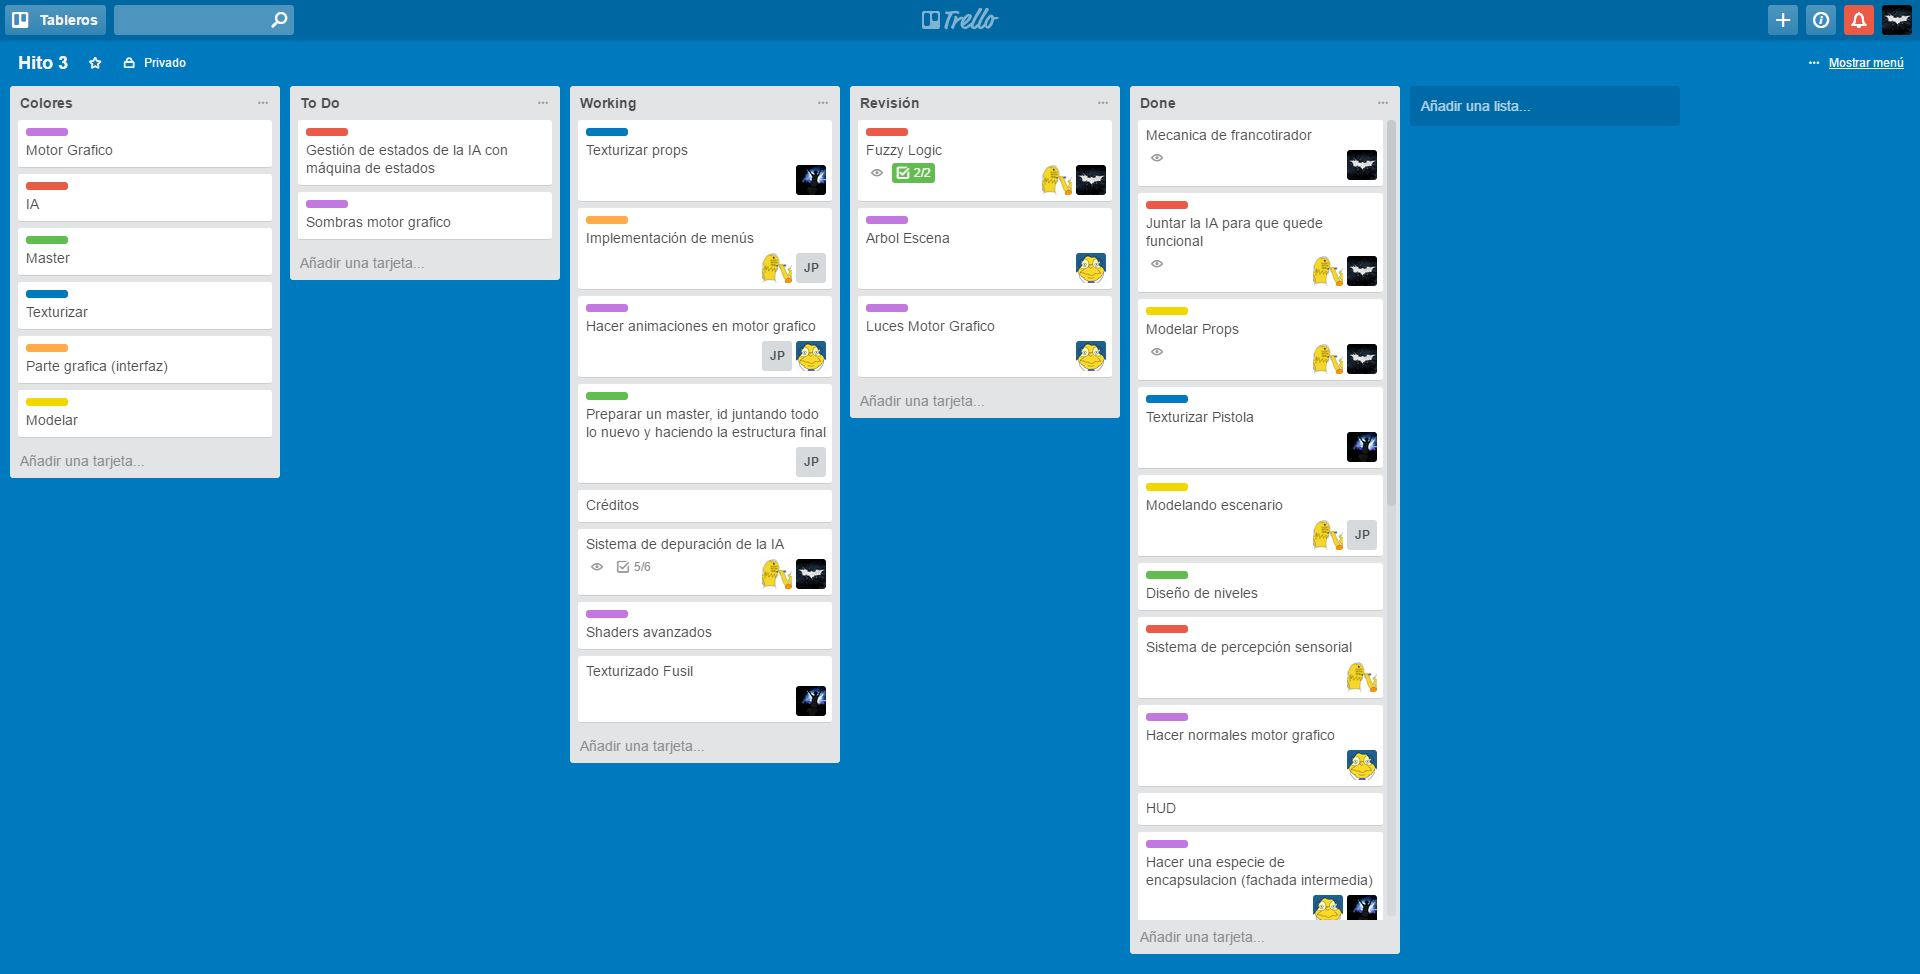
\includegraphics[scale=0.28]{imagenes/trello.jpg}
		\caption{Captura de pantalla de un tablero de \textit{Trello} de un proyecto anterior.}
		\label{trello}
	\end{center}
\end{figure}

El \ac{TFG} ha sido desarrollado usando la herramienta de gestión de proyectos \textit{Trello}, que nos permite crear tableros, etiquetas para las tareas y columnas en las que colocarlas. \textit{Trello} aporta una gran multitud de opciones con la que gestionar nuestros trabajos, como dividir las tareas en subtareas, clasificarlas por grupos o ponerles fechas límite o \textit{deadlines}.
\\

\textit{Trello} es una herramienta muy útil que he usado en anterioridad en otros trabajos y que resulta muy cómoda a la hora de gestionar el trabajo del proyecto.

\section{Control de versiones y repositorio}
	
Puesto que este es un trabajo individual no es necesario usar un sistema de control de versiones, no obstante, para mayor seguridad y para tener todo el contenido del proyecto disponible en Internet se ha decidido crear un repositorio en \textit{Github}.
De este modo siempre habrá una copia de seguridad disponible, además de que se puede volver a un momento anterior del proyecto si es necesario.
\\

El enlace del repositorio es el siguiente:
\\

\url{https://github.com/JoseLuisMunozP/TFG}

	
	
	
	
	
	
	
\begin{comment}


\begin{description}
\item[Índice de contenidos:] (obligatorio siempre) se incluirá un índice de las secciones de las que se componga el documento, la numeración de las 
divisiones y subdivisiones utilizarán cifras arábigas (según UNE 50132:1994) y harán mención a la página del documento donde se ubiquen.
\item[Índice de figuras:] si el documento incluye figuras se podrá incluir también un índice con su relación, indicando la página donde se ubiquen.
\item[Índice de tablas:] en caso de existir en el texto, ídem que el anterior.
\item[Índice de abreviaturas, siglas, símbolos, etc.:] en caso de ser necesarios se podrá incluir cada uno de ellos.
\end{description}
\item[Cuerpo del documento:] en el contenido del documento se da flexibilidad para su organización y se puede estructurar en las secciones que se considere. En todo caso obligatoriamente se deberá, al menos, incluir los siguientes contenidos:
\begin{description}
\item[Introducción:] donde se hará énfasis a la importancia de la temática, su vigencia y actualidad; se planteará el problema a investigar, así como el propósito o finalidad de la investigación.
\item[Marco teórico o Estado del arte:] se hará mención a los elementos conceptuales que sirven de base para la investigación, estudios previos relacionados con el problema planteado, etc.
\item[Objetivos:] se establecerá el objetivo general y los específicos.
\item[Metodología:] se indicará el tipo o tipos de investigación, las técnicas y los procedimientos que serán utilizados para llevarla a cabo; se identificará la población y el tamaño de la muestra así como las técnicas e instrumentos de recolección de datos.
\item[Resultados:] incluirá los resultados de la investigación o trabajo, así como el análisis y la discusión de los mismos.
\end{description}
\item[Conclusiones:] obligatoriamente se incluirá una sección de conclusiones donde se realizará un resumen de los objetivos conseguidos así como de los resultados obtenidos si proceden.
\item[Bibliografía y referencias:] se incluirá también la relación de obras y materiales consultados y empleados en la elaboración de la memoria del \ac{TFG}/\ac{TFM}. La bibliografía y las referencias serán indexadas en orden alfabético (sistema nombre y fecha) o se numerará correlativamente según aparezca (sistema numérico). Se empleará la familia 1 como tipo de letra. Podrá utilizarse cualquier sistema bibliográfico normalizado predominante en la rama de conocimiento, estableciéndose como prioritarios el sistema ISO 690, sistema \ac{APA}  o Harvard (no necesariamente en ese orden de preferencia). En esta plantilla Latex se propone usar el estilo \ac{APA} indicándolo en la línea correspondiente como 
\begin{verbatim}
\bibliographystyle{apalike}
\end{verbatim}


\item[Anexos:] se podrá incluir los anexos que se consideren oportunos.
\end{comment}



